\section{Experiment}
% We evaluate state-of-the-art language models based on efficiency and context window limits.


\subsection{Evaluation Settings}
Given an \textit{in-situ} user query and the user's interaction history up to a point in time, we evaluate models' ability to select the most appropriate response according to the current state of the user amonst four different choices. Only one of the choices fits the user's current status, and the other choices contain either irrelevant or outdated facts or preferences from the user.   
During evaluation, apart from the conversation history, the models have access to the basic demographic information of the user, including name, age, gender identity, racial identity, and occupation. The models do not have direct access to the user's other dynamic characteristics and personal history otherwise.

For selecting the most appropriate response, we evaluate models under both discriminative and generative settings. In the \textit{discriminative setting}, the models are presented with all four response choices denoted with (a), (b), (c) and (d) with random ordering among the choices. The model is asked to output the correct choice along with a brief explanation. 
In the \textit{generative setting}, the models still see one question at a time. We compute the log-sum of token probability of generating each option individually with length normalization, and select the option with the highest probability as the model response. We use the \textit{discriminative setting} for main evaluation (\S~\ref{ssec:discriminative},\S~\ref{ssec:long-context}, \S~\ref{ssec:rag}) and adopt the \textit{generative} setting in \S~\ref{ssec:geneartive}, as it requires access to logits over entire vocabulary during decoding, which is not available from most proprietary models. No LLM judges are involved in the evaluation process. 
% This is done by autoregressively appending the tokens of each candidate answer to the model’s output and recording the logit probabilities, and the final prediction is the one with the highest joint probability after length normalization. 
% We avoid LLM-as-a-judge in favor of more robust evaluation.


\subsection{Evaluating Language Models in Long-Context Settings}
\label{ssec:discriminative}
We first evaluate language models in the long-context setting, where the full user-LLM interaction history is provided as input to the models. Due to the length of the history, all models here were evaluated zero-shot, without demonstration examples of other histories and user queries.  
% long present comprehensive results on state-of-the-art language models used out-of-the-box with direct prompting, simulating practical, everyday user scenarios.
Our evaluation covers GPT-4.1, o4-mini, o3-mini, GPT-4.5, o1, GPT-4o, GPT-4o-mini, Gemini-2.0-Flash, Gemini-2.0-Flash-Lite, Gemini-1.5-Flash, DeepSeek-R1-671B, Llama-4-Maverick, Llama-3.1-405B, Claude-3.7-Sonnet, and Claude-3.5-Haiku~\citep{openai2025gpt45, openai2024o4mini, openai2025o3mini, openai2024o1, hurst2024gpt, team2024gemini, guo2025deepseek, grattafiori2024llama, anthropic2024claude3} on 128$k$-token context windows. We also evaluate models that support longer contexts—Llama-4-Maverick, Gemini-2.0-Flash, Gemini-2.0-Flash-Lite, and Gemini-1.5-Flash—on 1$M$-token context windows. 
We report the following findings:


\begin{figure}[t]
  \centering
  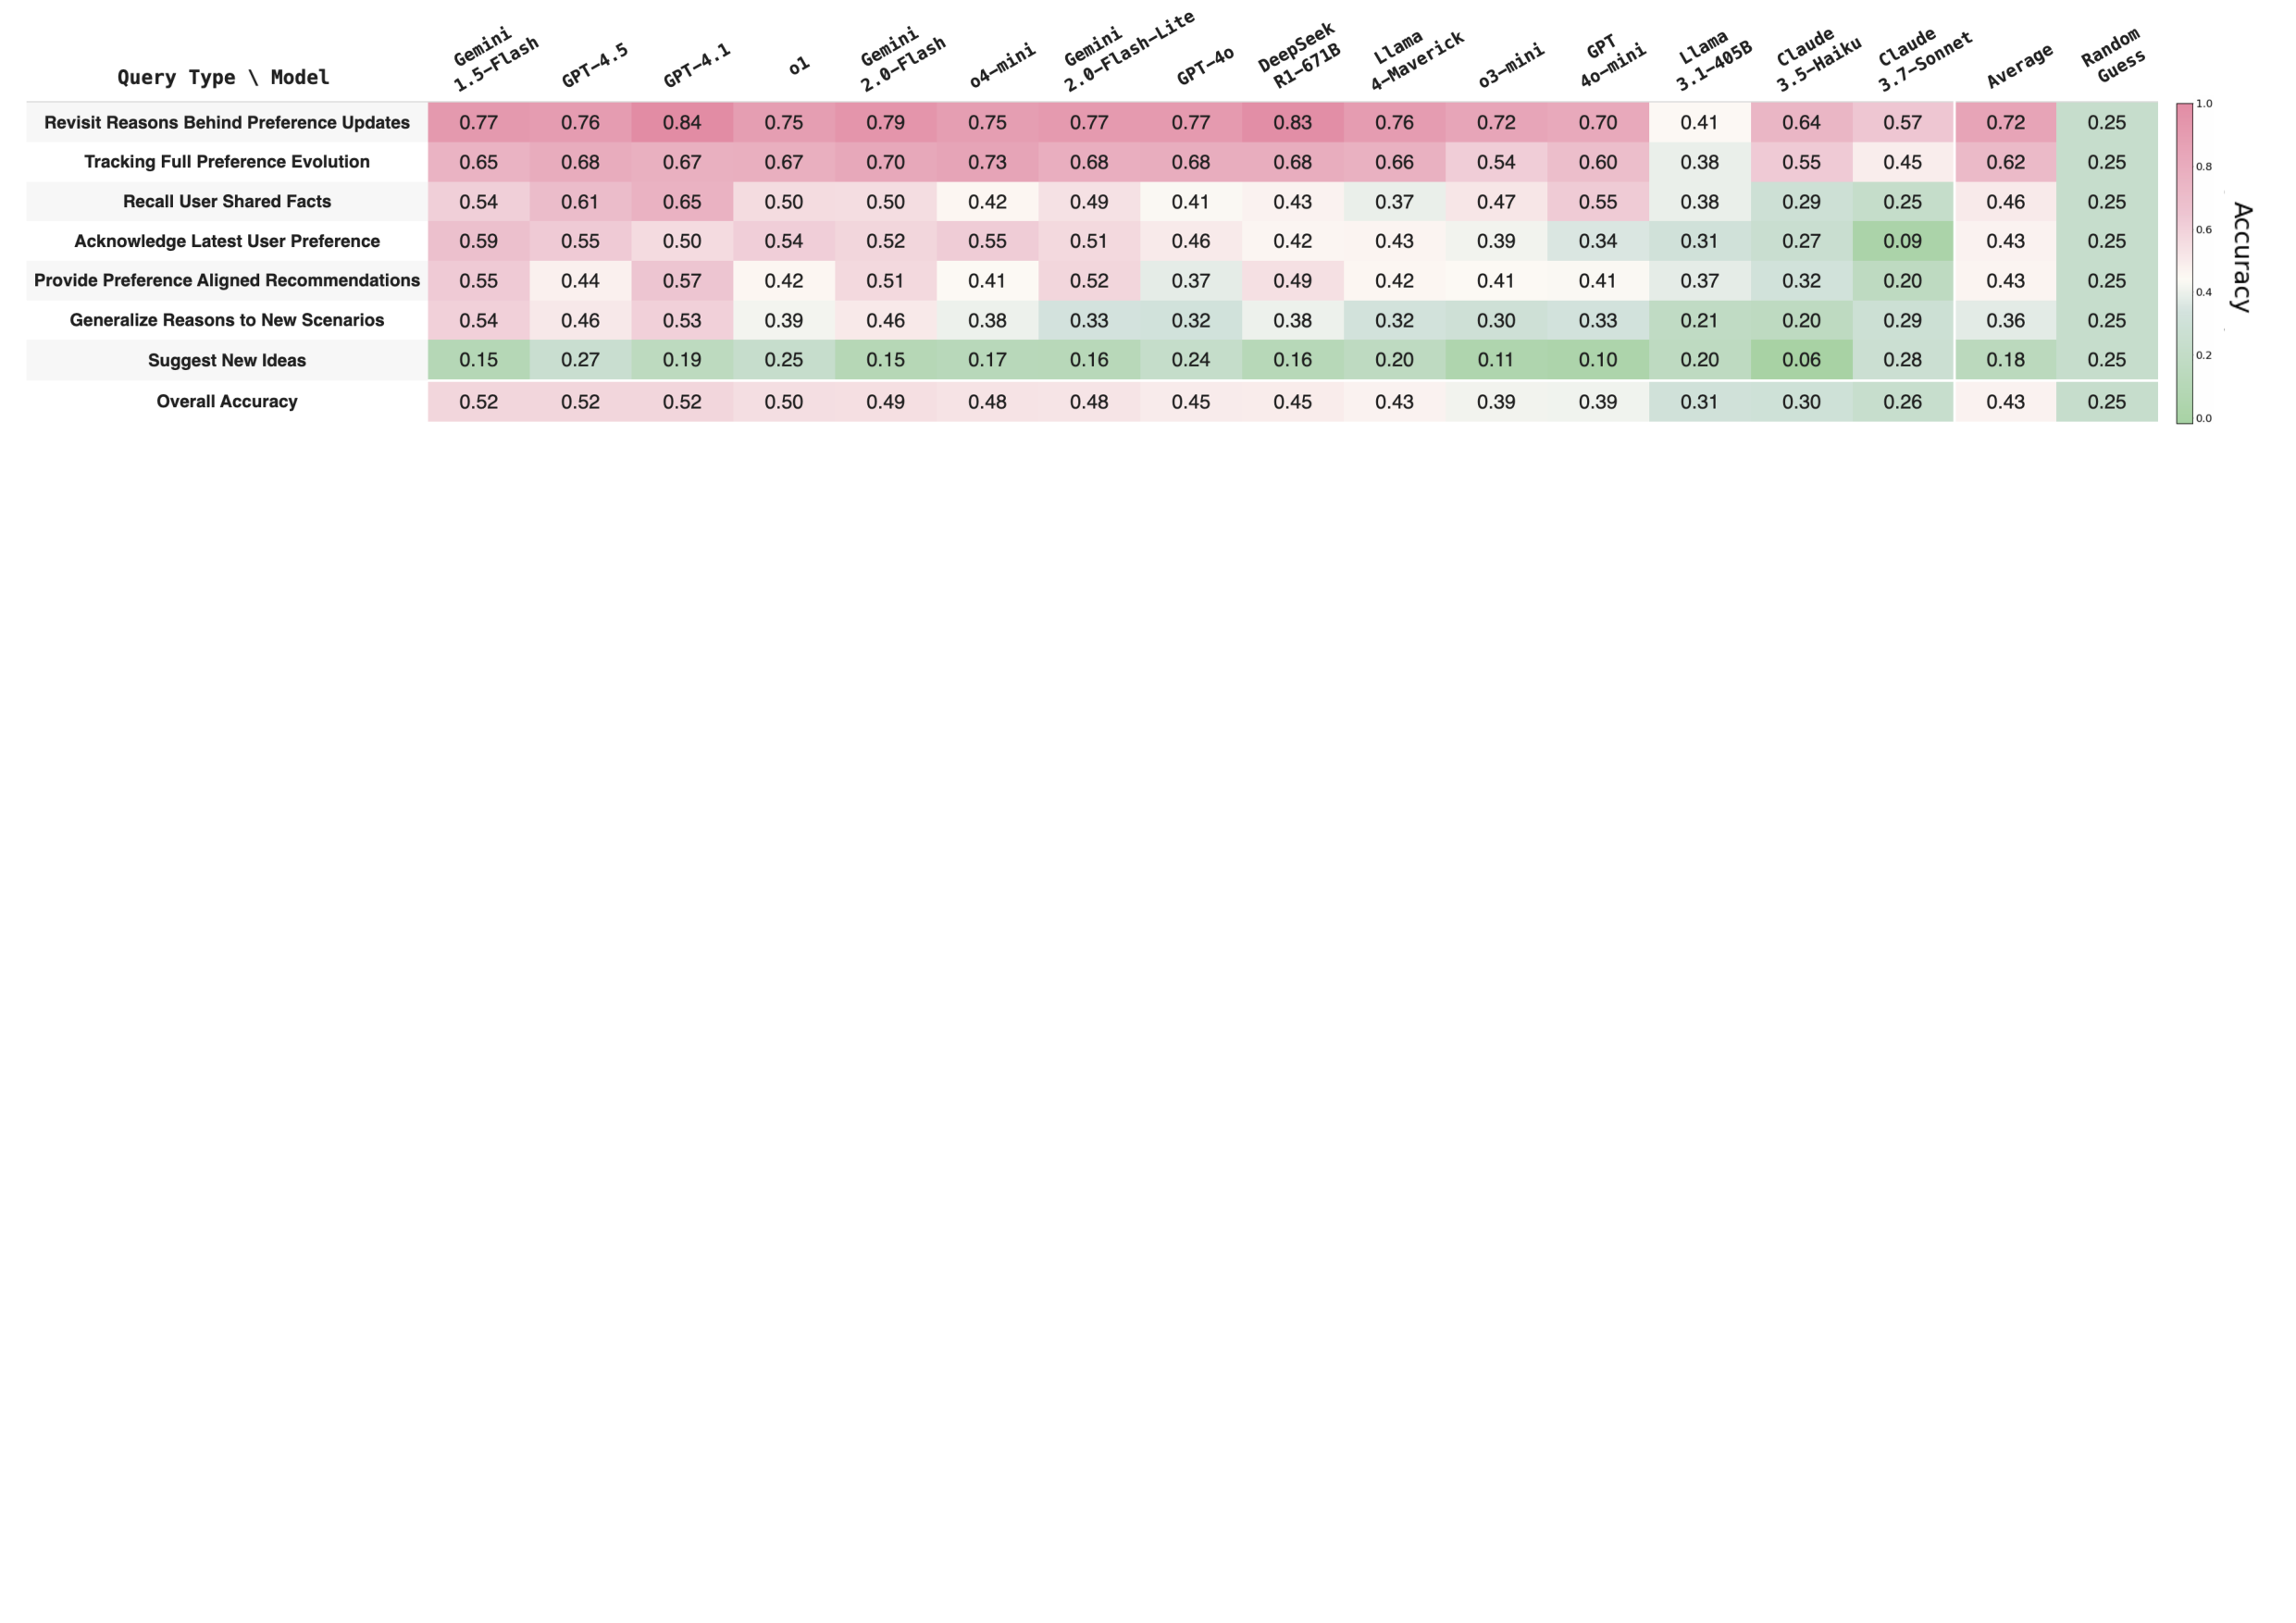
\includegraphics[width=1\linewidth]{figures/results_qa_types.pdf}
  \caption{Evaluation results across different models on 7 \emph{in-situ} query types. 
  % designed to test their ability to reason about user preferences, including acknowledging user facts, tracking preference changes, and generating aligned recommendations. 
  We observe models perform reasonably well at recalling user facts and preferences. However, models struggle at providing novel suggestions, or applying users' preferences in new scenarios.}
  % \vspace{-5mm}
  \label{fig:128k_qa_types}
\end{figure}

\begin{figure}[t]
  \centering
  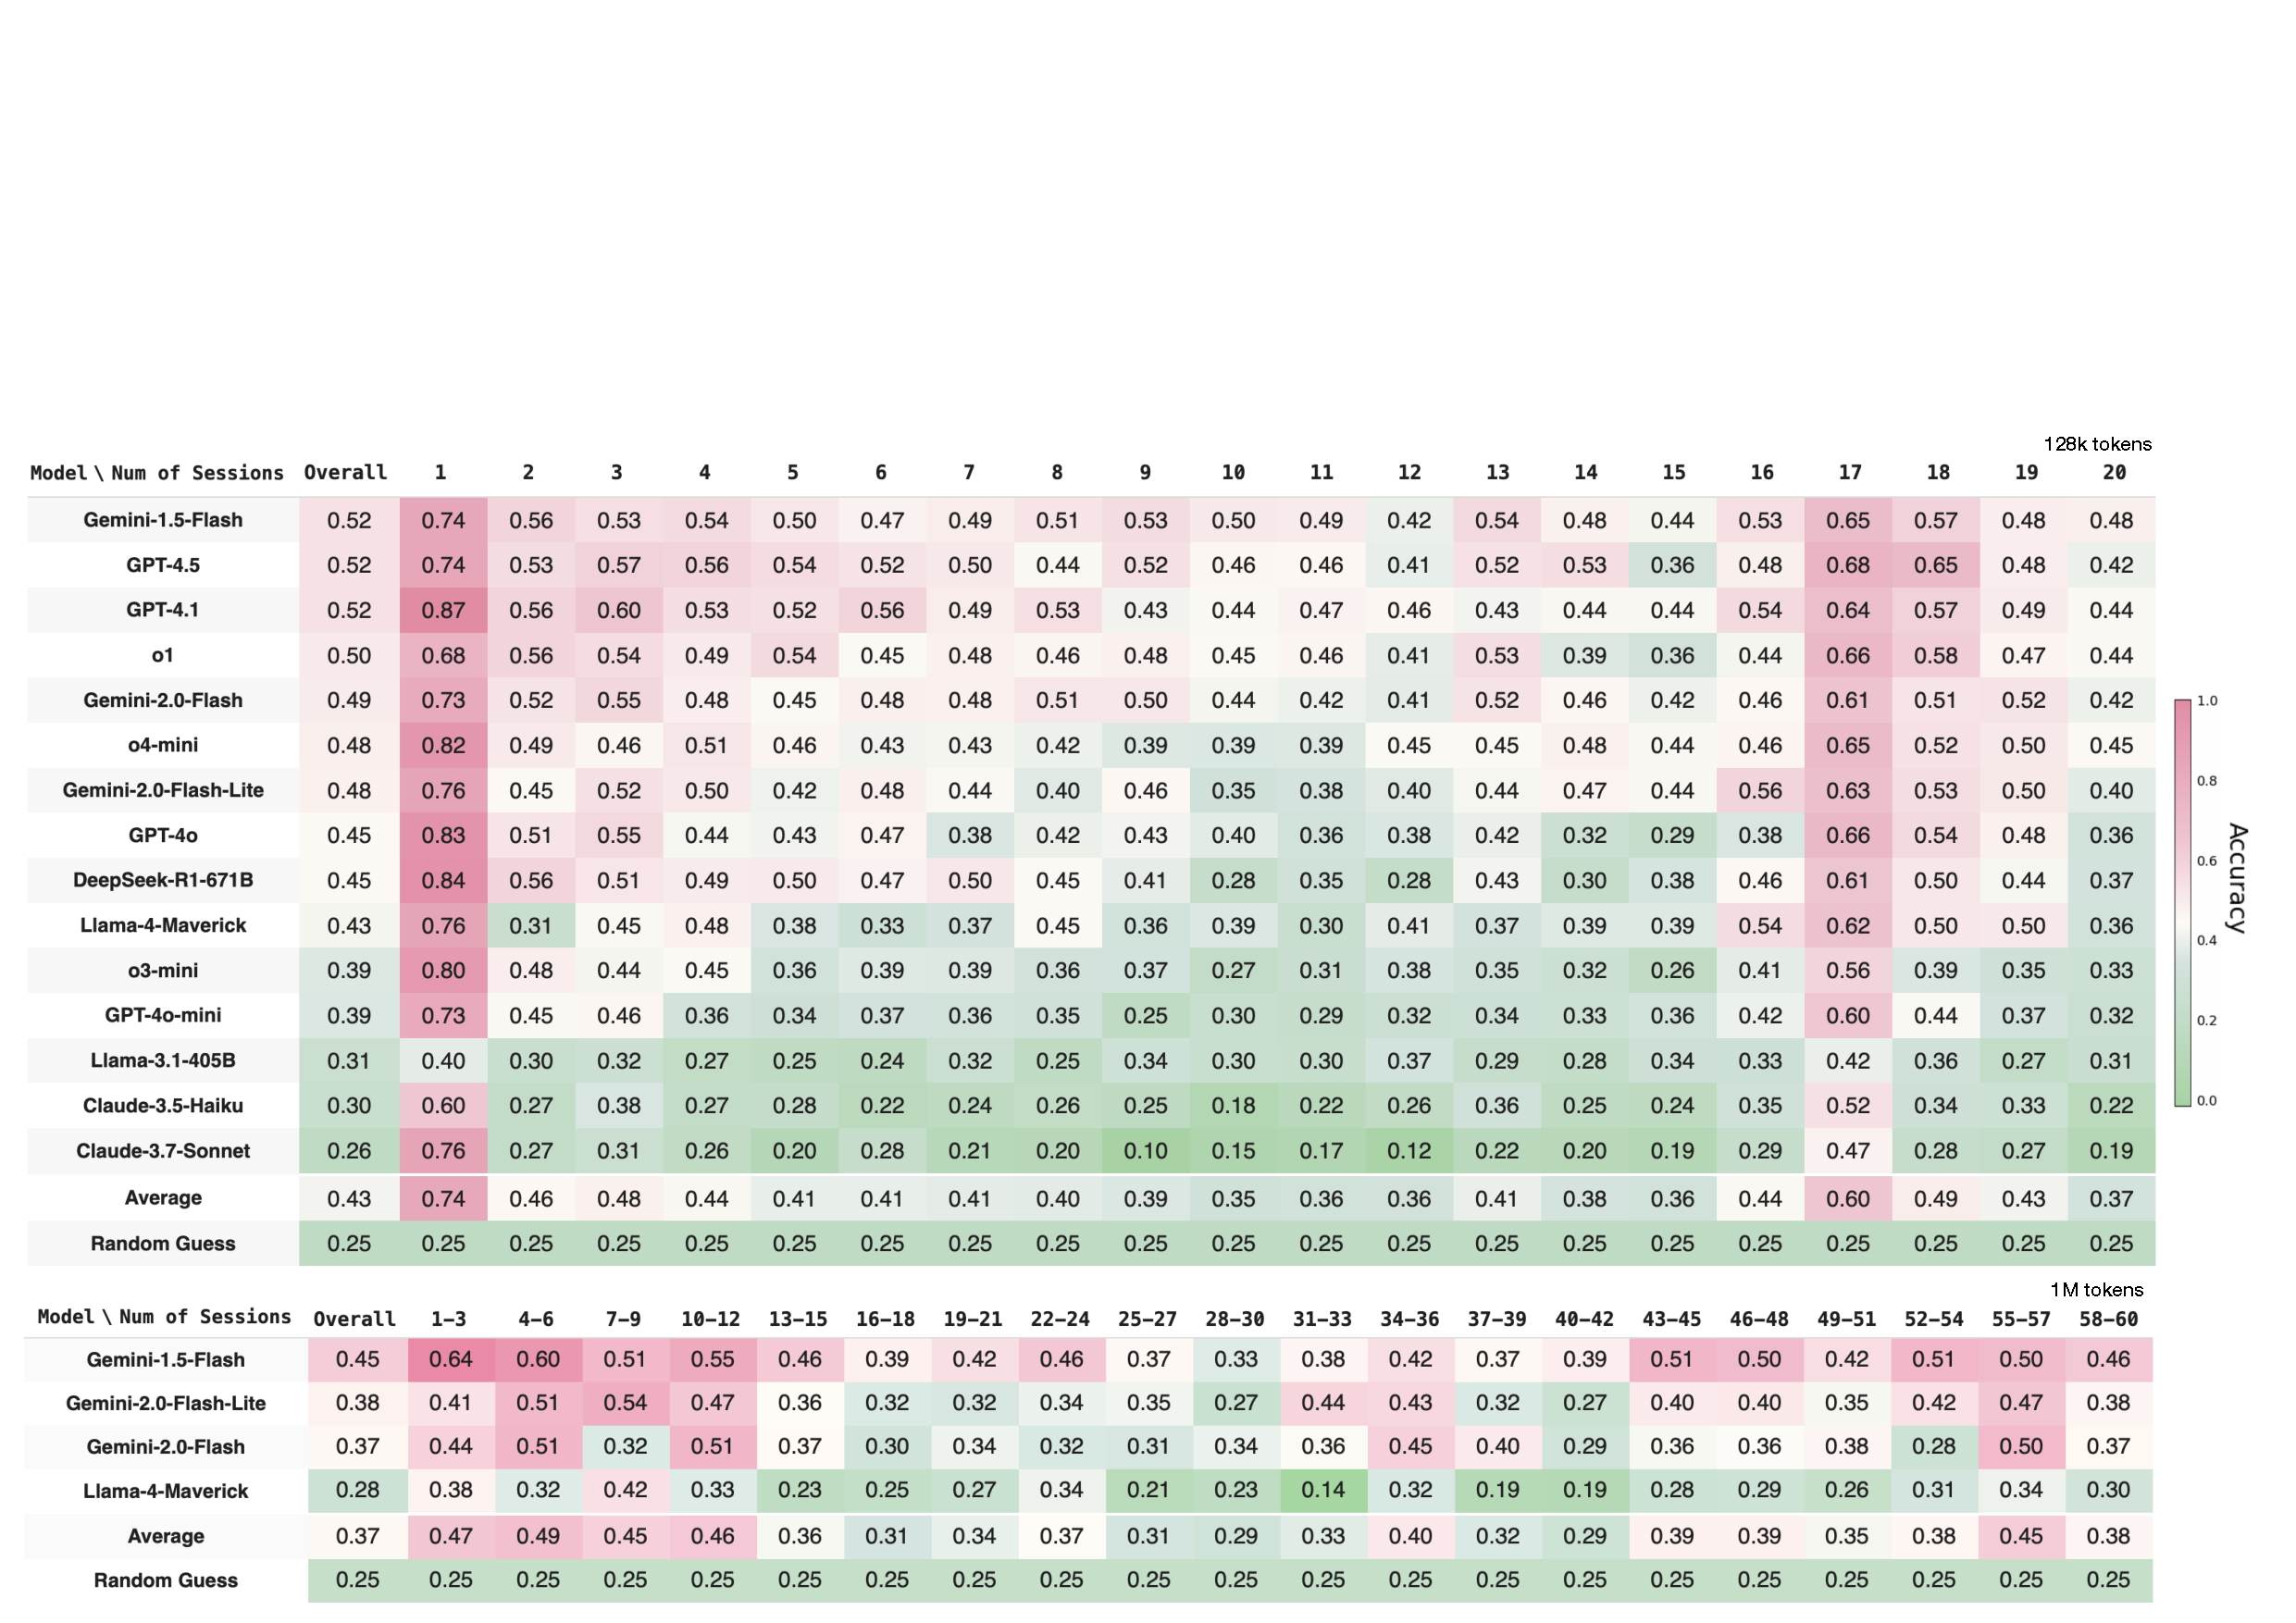
\includegraphics[width=1\linewidth]{figures/results_long_context.pdf}
  \caption{Model performances by number of sessions elapsed since most recent preferences were mentioned in long context. Top: up to 20 sessions/128k tokens; Bottom: up to 60 sessions/1M tokens. Long-context retrieval is important for personalization in practice.}
  % \vspace{-5mm}
  \label{fig:long_context}
\end{figure}




\paragraph{GPT-4.5, GPT-4.1, and Gemini-1.5 achieve the highest overall performance.}
Among leading foundation models, GPT-4.5 and Gemini-1.5 outperform others in overall accuracy. However, their performance still hovers around 52\% in a multiple-choice setting, highlighting substantial room for improvement. \textbf{Notably, reasoning models such as o1, o3-mini, o4-mini, and DeepSeek-R1-607B do not demonstrate competitive advantages over non-reasoning models in the personalization tasks we evaluate.}
% capabilities alone are insufficient for effective personalization, as demonstrated by advanced reasoning models such as o3-mini, o1, and DeepSeek-R1-607B. %We also observe a slight performance decline in the Gemini-2 series compared to Gemini-1.5. 

\paragraph{LLMs demonstrate reasonably good performance in recalling simple user facts.}
    For tasks involving the retrieval of static user information, such as previously mentioned items, activities, or reasons behind preference changes where the reasons themselves won't change, most LLMs have a reasonable chance of succeeding.
    
\paragraph{Incorporating the latest user preference into responses is more challenging than recalling the change in user profile.} We observe that models struggle to incorporate the latest preference or state of the user in responses. Surprisingly, models generally get higher performance when asked to recall how the user preferences evolve over time. 
We observe that asking the model to iterate through all preference updates may encourage it to think through the preference evolutions, often making the task easier.
    
\paragraph{Models fall short on generating new ideas or providing suggestions in new scenarios.}
    As shown in Figure~\ref{fig:128k_qa_types}, tasks such as \textit{"Suggest New Ideas}", \textit{"Provide Preference-Aligned Recommendations"}, and \textit{"Generalize Reasons to New Scenarios"} yield the lowest performance across all models, highlighting the challenge of generating personalized responses in novel contexts—particularly when identifying new facts.


\subsection{Effect from the Position of User Information in Interaction History}
\label{ssec:long-context}
To understand how the model performance is affected by the position in which the relevant user facts or preferences appear in the conversation history, we report the model performance by the session in which the relevant user information appears in the history. The results are shown in Figure~\ref{fig:long_context}. Generally, we observe that the model performs better when the relevant information appears in the earler or later sessions of the conversation history. The findings here generally echo previous findings on long-context inputs to models, where context information tends to get ``lost in the middle'' \citep{liu2024lost, wu2024longmemeval}.     

    % As shown in Figure~\ref{fig:long_context}, personalization under long context windows remains difficult, particularly for user information that appears far from the end of the context, indicating that long-context retrieval is important for achieving strong personalization in practice.
    



% \begin{table*}[ht]
% \centering
% \small
% \resizebox{\textwidth}{!}{%
% \begin{tabular}{lcccccccc}
% \toprule
% \textbf{Model} & 
% \makecell[c]{\textbf{Overall}} & 
% \makecell[c]{\textbf{Revisiting} \\ \textbf{Previous} \\ \textbf{Reasons}} & 
% \makecell[c]{\textbf{Tracking} \\ \textbf{Full} \\ \textbf{Evolution}} & 
% \makecell[c]{\textbf{Incorporating} \\ \textbf{Latest} \\ \textbf{Preference}} & 
% \makecell[c]{\textbf{Incorporating} \\ \textbf{User Shared} \\ \textbf{Facts}} & 
% \makecell[c]{\textbf{Preference} \\ \textbf{Aligned} \\ \textbf{Recommendations}} & 
% \makecell[c]{\textbf{Generalizing} \\ \textbf{Reason to} \\ \textbf{New Scenarios}} & 
% \makecell[c]{\textbf{Identifying} \\ \textbf{Facts Not} \\ \textbf{Shared Before}} \\
% \midrule
% Gemini-1.5-Flash        & \textcolor{red}{\textbf{0.52}} & 0.77 & 0.65 & 0.59 & 0.54 & 0.55 & \textcolor{red}{\textbf{0.54}} & 0.15 \\
% GPT-4.5                 & \textcolor{red}{\textbf{0.52}} & 0.76 & 0.68 & \textcolor{red}{\textbf{0.76}} & \textcolor{red}{\textbf{0.61}} & 0.44 & 0.46 & \textcolor{red}{\textbf{0.27}} \\
% o1                      & 0.50 & 0.75 & 0.67 & 0.54 & 0.50 & 0.42 & 0.39 & 0.25 \\
% Gemini-2.0-Flash        & 0.49 & 0.79 & \textcolor{red}{\textbf{0.70}} & 0.52 & 0.50 & 0.51 & 0.46 & 0.15 \\
% Gemini-2.0-Flash-Lite   & 0.48 & 0.72 & 0.68 & 0.50 & 0.51 & \textcolor{red}{\textbf{0.52}} & 0.33 & 0.16 \\
% GPT-4o                  & 0.45 & 0.77 & 0.67 & 0.46 & 0.41 & 0.37 & 0.32 & 0.24 \\
% DeepSeek-R1-67B         & 0.45 & \textcolor{red}{\textbf{0.83}} & 0.68 & 0.42 & 0.43 & 0.49 & 0.38 & 0.16 \\
% o3-mini                 & 0.39 & 0.76 & 0.60 & 0.40 & 0.40 & 0.41 & 0.31 & 0.14 \\
% GPT-4o-mini             & 0.39 & 0.70 & 0.60 & 0.34 & \textcolor{red}{\textbf{0.55}} & 0.41 & 0.33 & 0.10 \\
% LLaMA-3-405B            & 0.31 & 0.41 & 0.38 & 0.31 & 0.38 & 0.37 & 0.21 & 0.20 \\
% Claude-3.5-Haiku        & 0.30 & 0.65 & 0.34 & 0.24 & 0.29 & 0.20 & 0.22 & 0.06 \\
% Claude-3.7-Sonnet       & 0.26 & 0.57 & 0.45 & 0.09 & 0.25 & 0.20 & 0.29 & 0.09 \\
% \midrule
% \textbf{Average Accuracy} & \textbf{0.420} & \textbf{0.694} & \textbf{0.548} & \textbf{0.456} & \textbf{0.434} & \textbf{0.404} & \textbf{0.359} & \textbf{0.163} \\
% Random Guess            & 0.25 & 0.25 & 0.25 & 0.25 & 0.25 & 0.25 & 0.25 & 0.25 \\
% \bottomrule
% \end{tabular}
% }
% \caption{Prompt: Model performance across multiple reasoning skills. "Overall" is placed first; other columns are sorted by average accuracy (excluding Random Guess) in descending order. Maximum per column is bold and red. Average accuracy row is shown just above Random Guess.[\textcolor{red}{TODO}: transform other result tables using this prompt]}
% \label{tab:multi_skill_eval_sorted_desc}
% \end{table*}



% \begin{figure}[t]
%   \centering
%   \includegraphics[width=1\linewidth]{figures/results_1m_sessions.png}
%   \caption{TODO}
%   % \vspace{-5mm}
%   \label{fig:1m_sessions}
% \end{figure}


\subsection{Evaluation with External Memory Modules}
\label{ssec:rag}

% \begin{figure}[t]
%   \centering
%   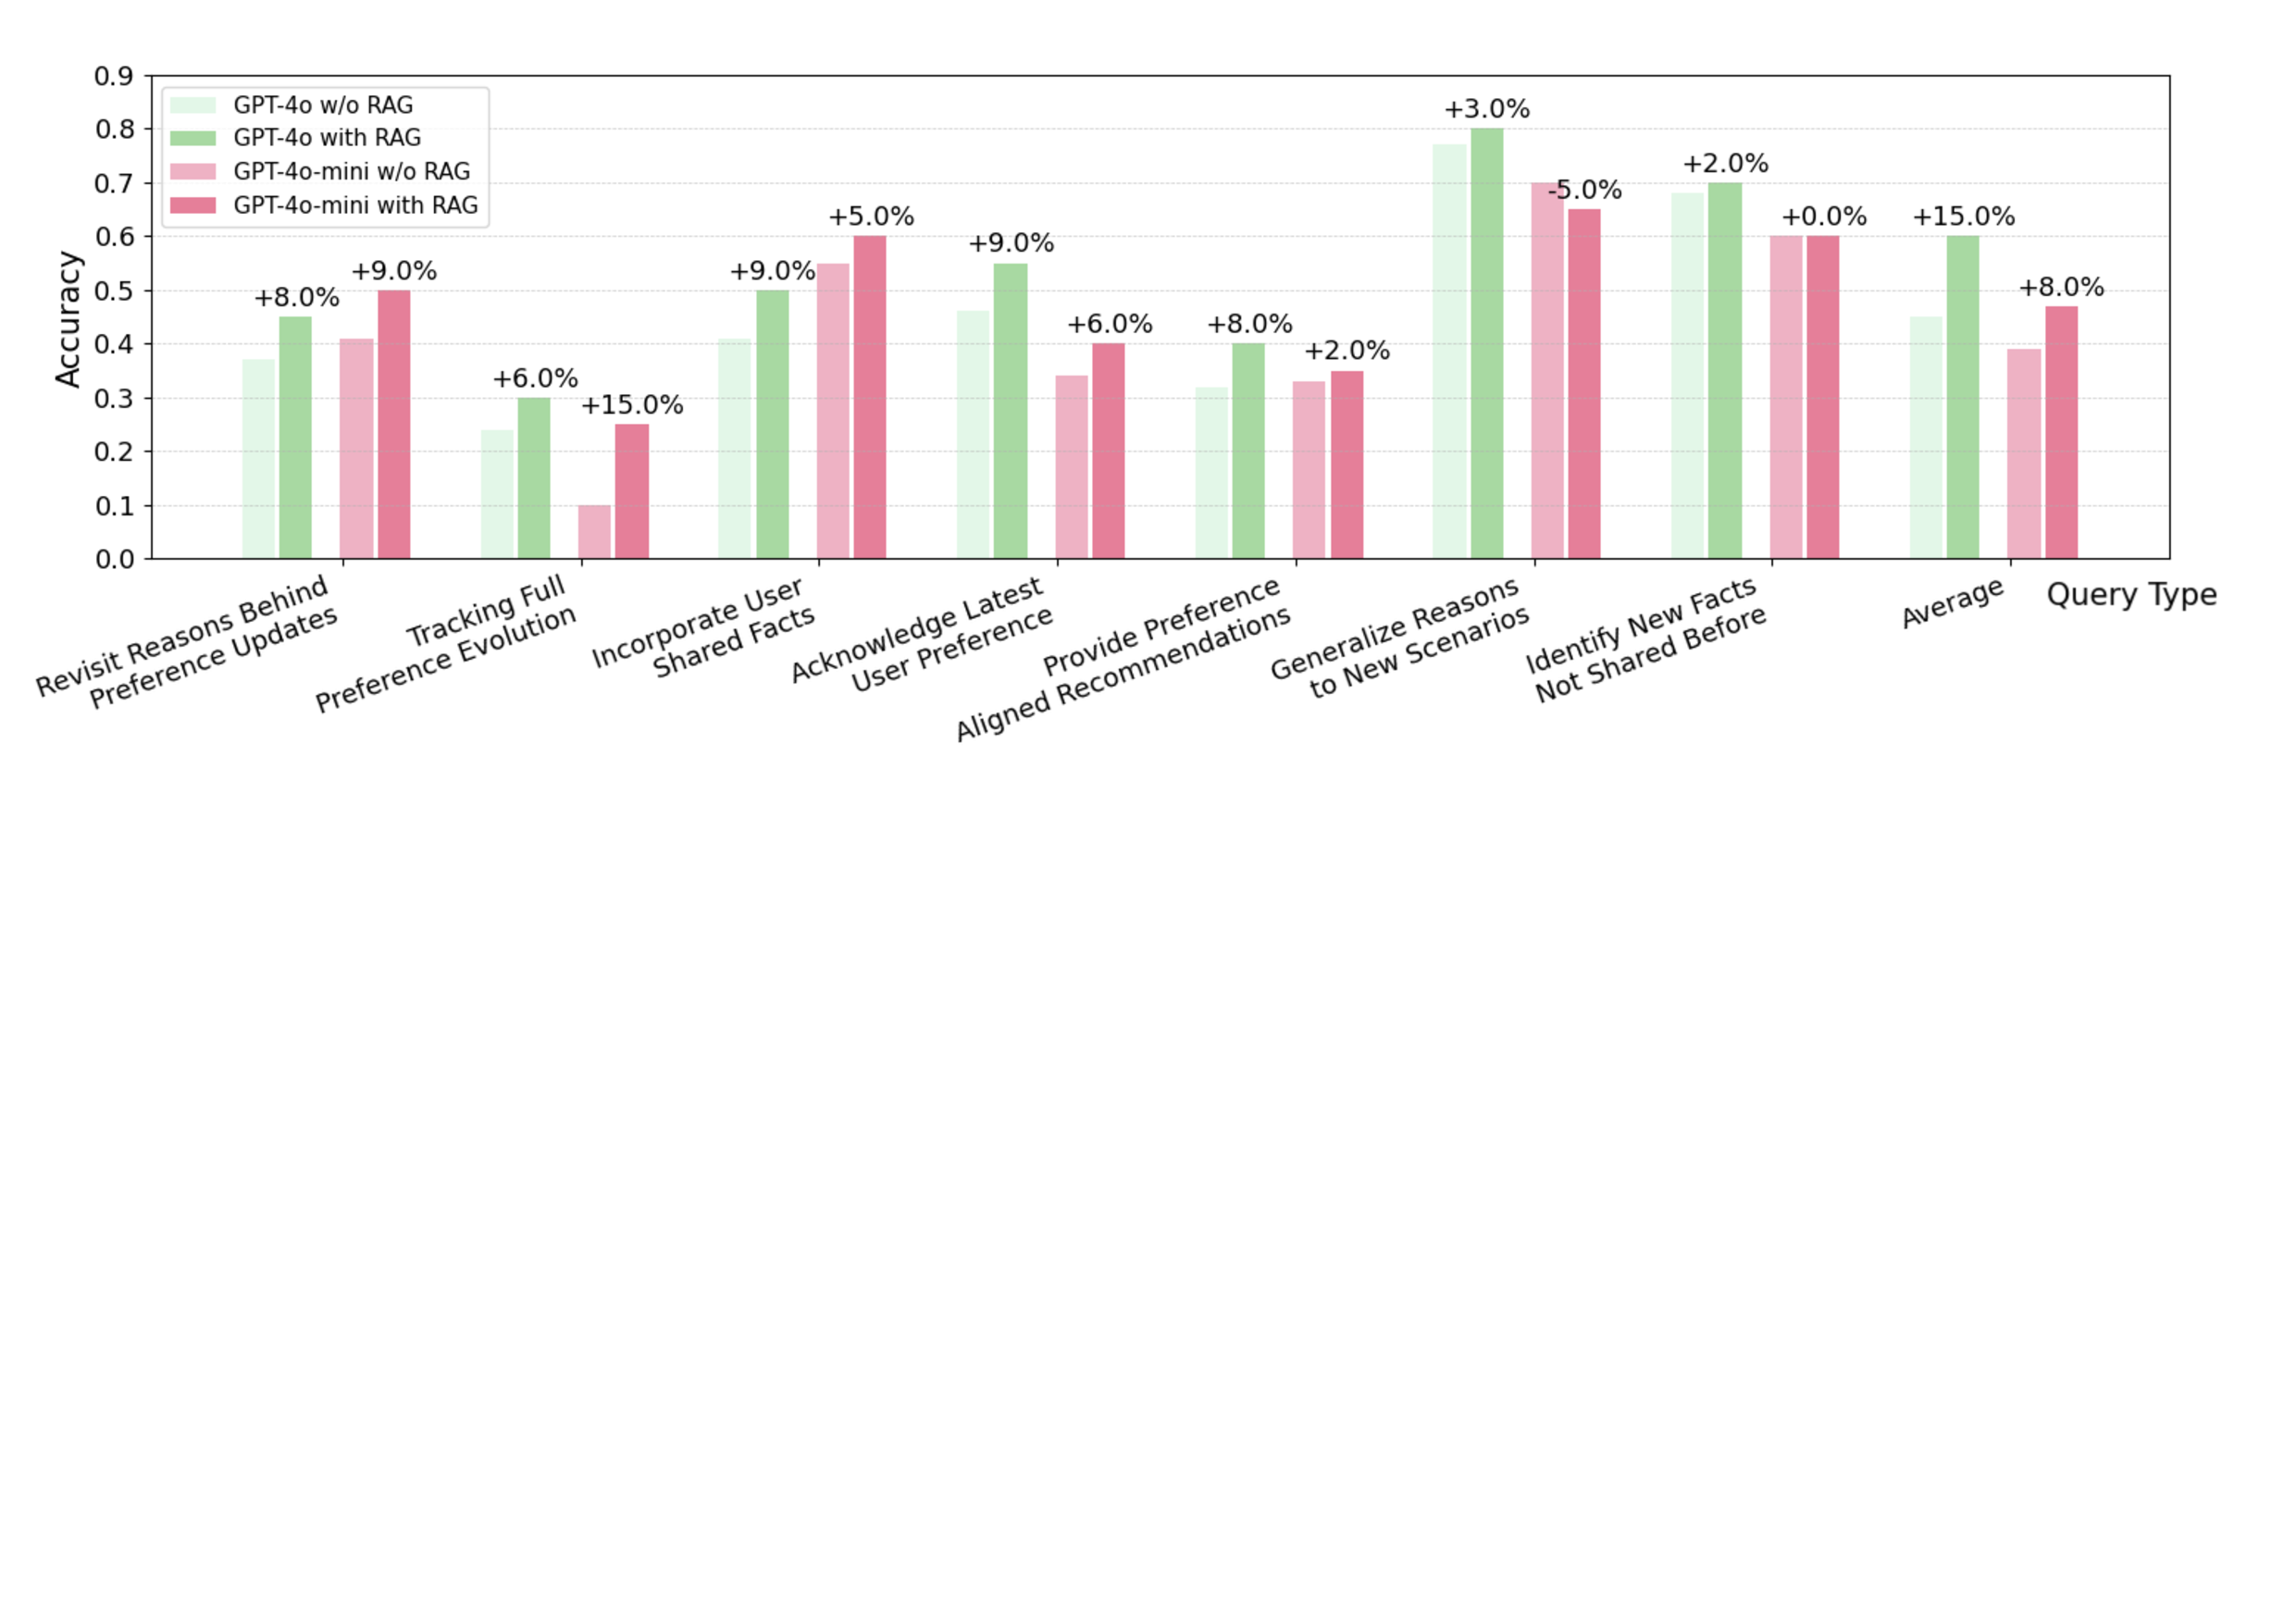
\includegraphics[width=1\linewidth]{figures/rag_128k.pdf}
%   \caption{Performance on the different question types for GPT-4o and GPT-4o-mini on the 128k context setting, and comparing with RAG to without RAG. We observe that overall RAG improves accuracy across types and models. Most notable boosts are for `Tracking Full Preference Evolution'. However, as expected, it fails to assist in the types involving new information.}
%   % \vspace{-5mm}
%   \label{fig:rag_128k}
% \end{figure}

\begin{figure}[t]
  \centering
  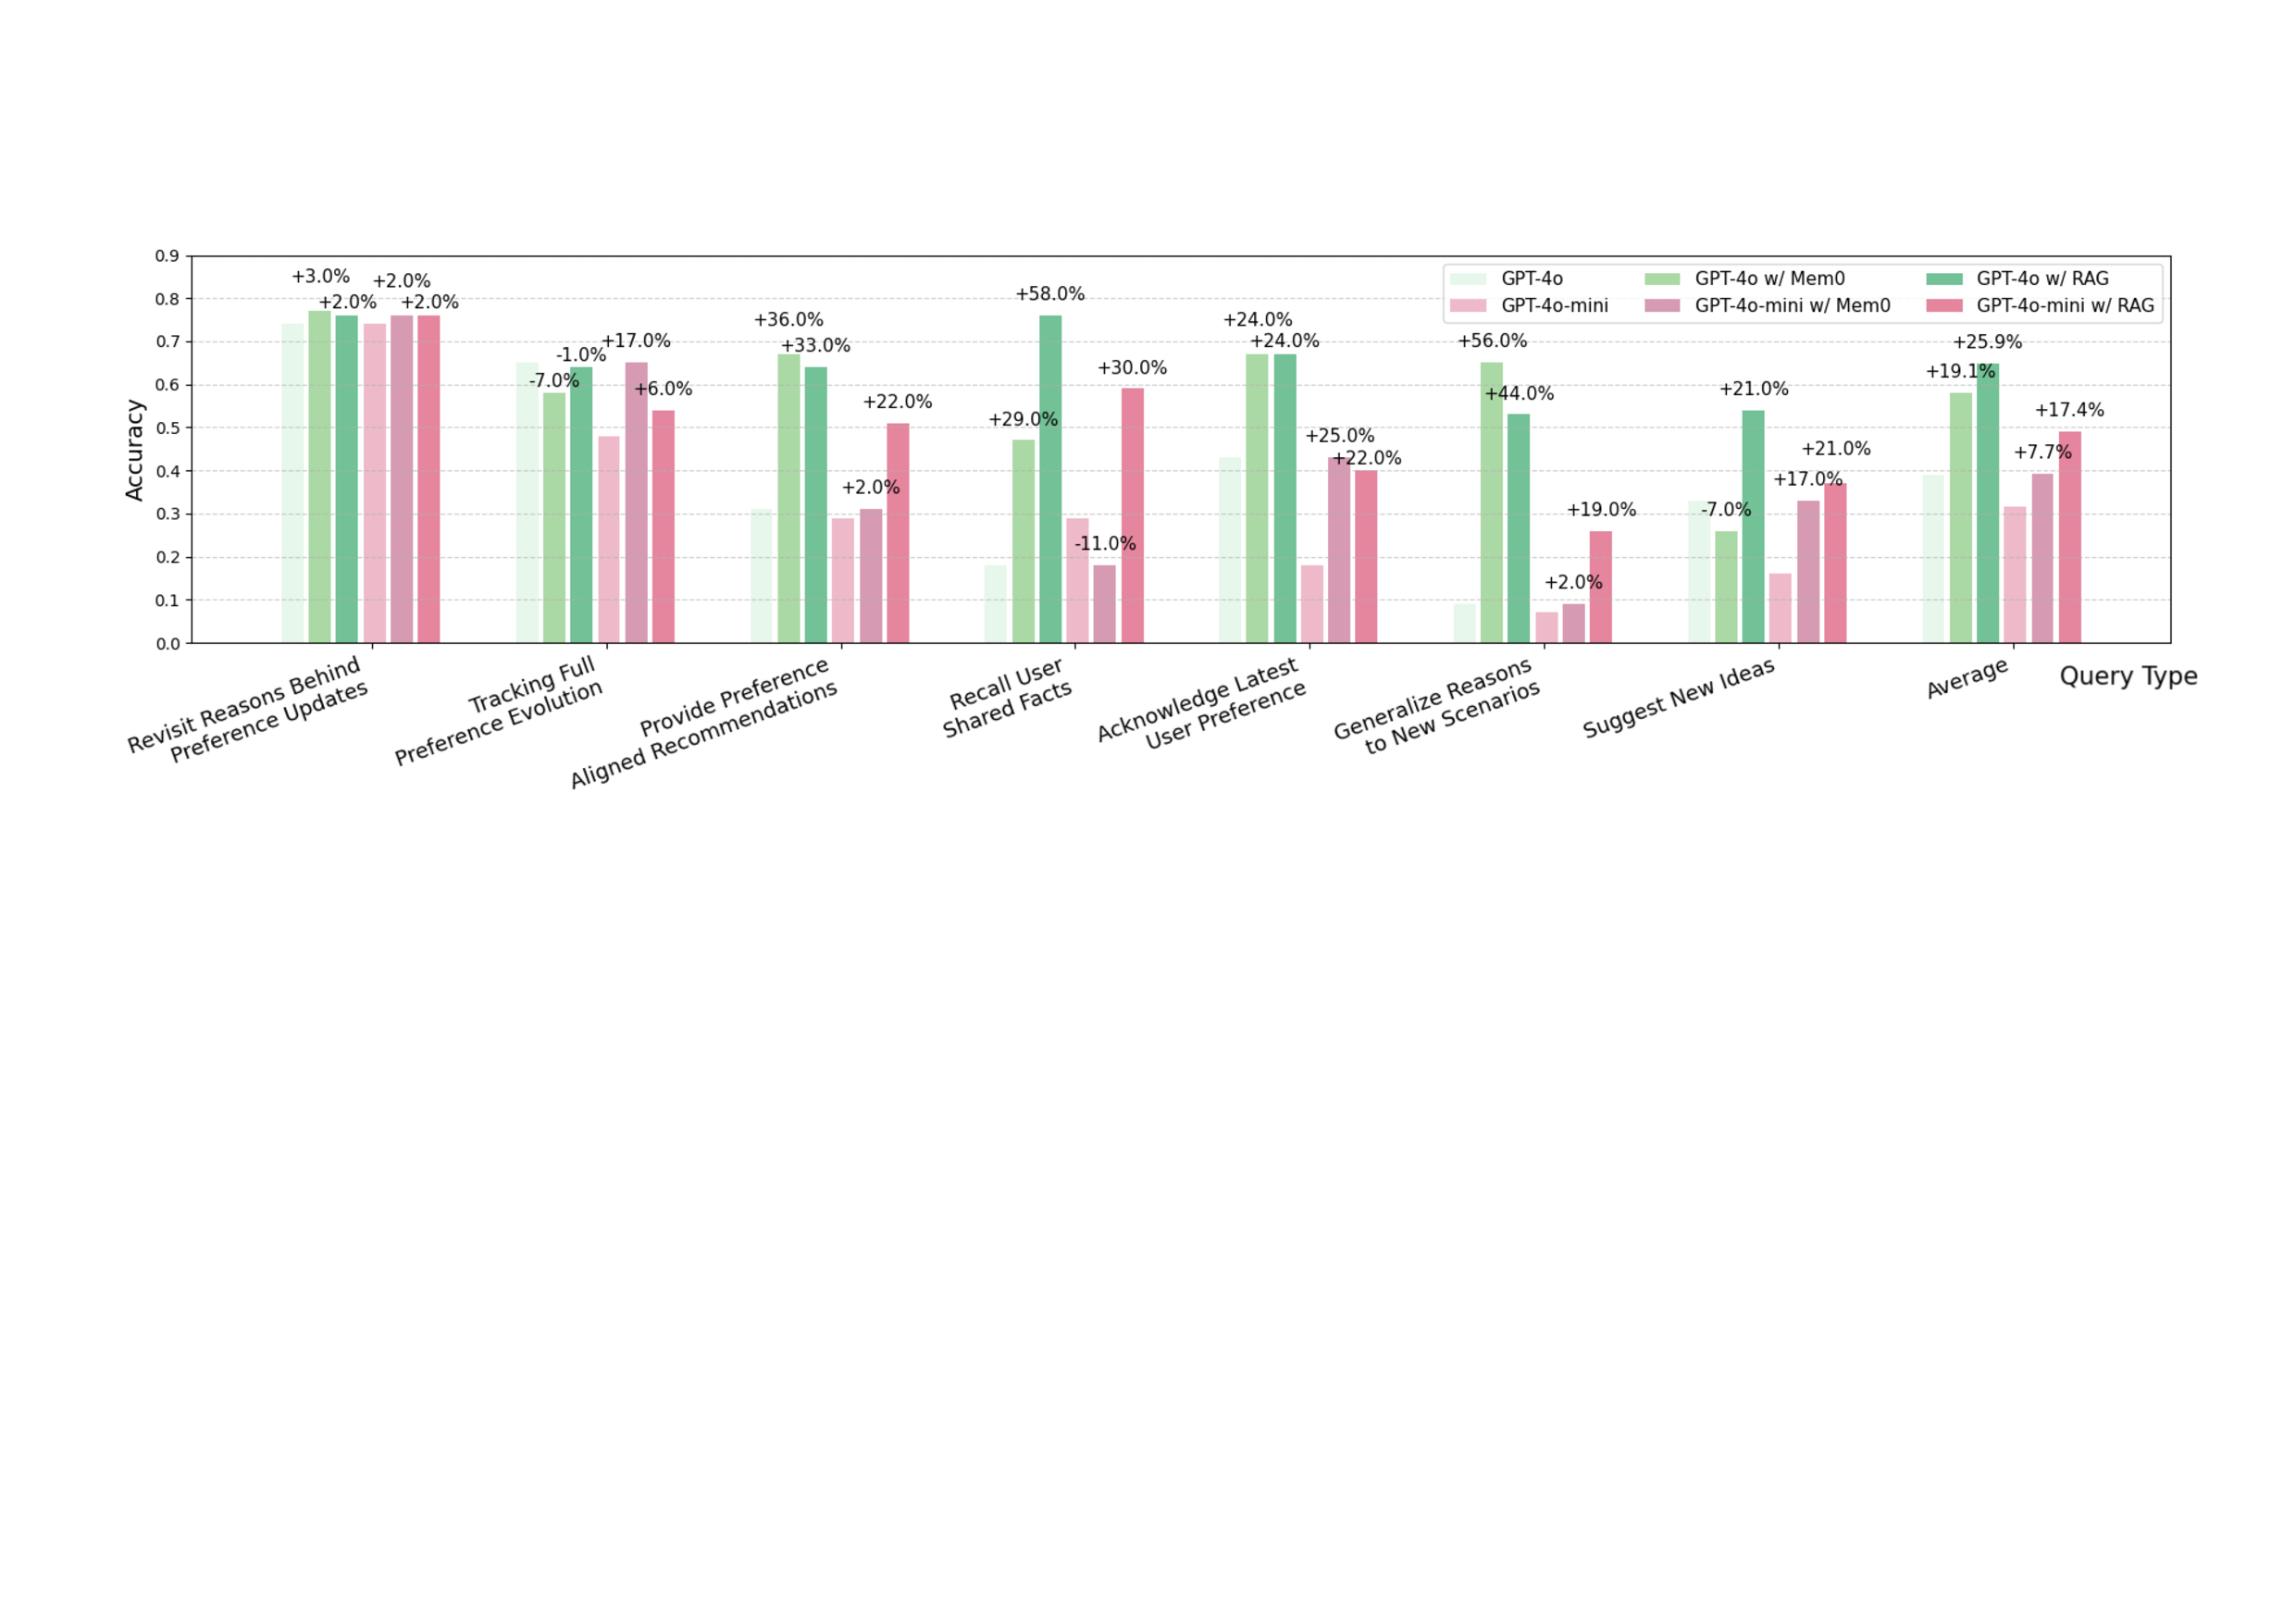
\includegraphics[width=1\linewidth]{figures/rag_mem0_32k.pdf}
  \caption{Performance on different question types for GPT-4o and GPT-4o-mini with 32k-token contexts. We compare vanilla models to the ones with Mem0 and RAG setups.}
  \vspace{-2mm}
  \label{fig:rag_mem0_32k}
\end{figure}




% , including Retrieval Augmented Generation (RAG) and external memory modules. 

% \subsubsection{RAG-based Evaluation}
% \paragraph{Models} 
% \paragraph{Approaches}
We evaluate whether using a retriever to identify relevant information in the history will help improve model's performance.
% To understand the impact of retrieval modules,
We evaluate two external memory approaches—RAG~\citep{lewis2020retrieval} and Mem0~\citep{mem0}—against vanilla LLMs. For these experiments, we consider only the GPT-4o and GPT-4o-mini models. We show their latency in Appendix~\ref{app:latency}.

For RAG, we consider a straightforward implementation that retrieves the top five most relevant messages per question using dense BGE-M3 embeddings~\citep{chen2024bge}. For Mem0 which provides an additional memory layer to LLMs, we iteratively build a memory database using LLM-generated facts over each turn. At inference, we retrieve the top 5 relevant facts per question. For efficiency, we use 32k-token contexts for evaluation.



% We first consider a straightforward implementation of Retrieval Augmented Generation (RAG). Given an input context we retrieve the 5 most relevant messages with respect to a given question. We use BGE-M3 embeddings with the dense retrieval approach~\citep{chen2024bge}. 

% For Mem0 that provides an additional memory layer to LLMs, we iteratively build a memory database using LLM-generated facts over each turn. At inference, we retrieve the top 5 relevant facts per question. 


% evaluate GPT-4o and GPT-4o-mini models, both with and without RAG modules, across context windows of 32k and 128k tokens. For our RAG implementation, we adopt a straightforward method: for each question, we retrieve the five most similar messages from the context window using dense M3 embeddings \citep{chen2024bge}. These retrieved messages are then provided to the LLM alongside the question and its answer options to produce predictions.

% We also consider Mem0, an open-source package that adds a memory layer for LLMs \citep{mem0}. It operates by using LLM prompts to dynamically update a database of user facts; we do so iteratively over each turn in the context. Similarly to RAG, we retrieve the top 5 most relevant facts with respect to a given question.

% We compare the above two external memory approaches with the default full context setting, which passes the entire context alongside quesitons and options to LLMs.

% \paragraph{Results} 
\paragraph{Retriever-based memory module can improve model performance. }
Overall, external memory modules significantly improve accuracy for both models. Notably, \textit{Recall User-Shared Facts} and \textit{Generalize to New Scenarios} benefit the most, highlighting the effectiveness of retrieval in factual tasks. In contrast, \textit{Revisit Reasons Behind Preference Updates} shows smaller gains. RAG consistently outperforms Mem0 across most question types, although Mem0 is more computational expensive, suggesting that retrieving semantically similar messages is more effective for personalized reasoning.


% We show the performance of different approaches with a 32K context setting in Table \ref{fig:rag_mem0_32k}. Overall, using an external memory module significantly increases performance in both LLMs. Notably, performance on Recall User-Shared Facts and Generalize to New Scenarios questions shows a substantial improvement compared to the full context method, demonstrating effectiveness in handling factual questions. On the other hand, Revisit Reasons Behind Preference Updates and Track Full Preference Evolution only show marginal gains or even decreased accuracy, which indicates a need for broader memory coverage. Notably, RAG outperformed Mem0 in most of the question types, suggesting that retrieving semantically close messages to questions can be effective in solving personalized problems. Furthermore, gpt-4o with RAG on a 128K context setting achieved the highest accuracy of 59.8\%, demonstrating robustness under extremely high context lengths.

% \subsubsection{Memory-Augmented Evaluation}
% \paragraph{Models} 
% We explore Mem0~\citep{mem0}—an additional memory layer for language models—using GPT-4o and GPT-4o-mini within a 32$k$ token context window.
% \paragraph{Results}

\subsection{Evaluation of Language Models in Generative Settings}
\label{ssec:geneartive}
In real-world use cases, the chatbots do not have access to the potential options of responses during inference. For such reason, we additionally evaluate models on the more realistic \emph{generative} settings, where the model sees only one option at a time, and the best response is selected by the joint sequence probability of options from model predictions.    

% While multiple-choice question answering (MCQ) tasks effectively assess a model's ability to select appropriate responses from predefined options, they do not fully reflect realistic user interactions with language models. In practical scenarios, users rarely present multiple candidate answers but instead engage in natural conversations. To bridge this gap, we propose to evaluate whether LLMs can generate personalized responses directly in response to user queries rather than prompting the model to choose explicitly from given candidates 


\paragraph{Approaches.} 
Given the user-LLM history and in-situ user query, we compare the joint sequence probabilities by taking the log-sum of the token-level probability of each response option. 
% for each query-answer pair. 
Specifically, given a conversation history (denoted as \( \mathcal{C} \)) and the user query (\( q \)), we evaluate each candidate response $r_{i \in \{1, 2, 3, 4\}}$, consisting of tokens \( \{x_i^1, x_i^2, \dots, x_i^{T_l}\} \) of total token length $l$. Due to the \textit{autoregressive} nature of causal language models, the joint log probability for each query-answer pair is computed by summing the conditional log probabilities of each token given its preceding context, formalized as 
% $\log P(r_i \mid \mathcal{C}, q) = \sum_{t=1}^{T_i} \log P(x_i^t \mid \mathcal{C}, q, x_i^1, \dots, x_i^{t-1})$.
\vspace{-1mm}
\[
\log P(r_i \mid \mathcal{C}, q) = \sum_{t=1}^{T_i} \log P(x_i^t \mid \mathcal{C}, q, x_i^1, \dots, x_i^{t-1})/T_i
\]
\vspace{-3mm}

As the method requires logarithmic probability of output tokens over the entire vocabulary, which is often not available in proprietary models, we evaluate open-weight models—LLaMA-3.1–70B, LLaMA-3.1–8B, and DeepSeek-Distill-LLaMA–8B. Due to constraints in computation resources, we only evaluate the models on the 10-session version of the benchmark, which includes around 32$k$-tokens per session.

\paragraph{Results.} As shown in Figure \ref{fig:generative}, we observe the similar trend to our \emph{discriminative} evaluation results in terms of difficulty by different user query types. Models get reasonably good performance on recalling facts and tracking preference changes, while giving new suggestions and generalizing to new scenarios are still the most challenging types of queries for models. Interestingly, when comparing the same model, specifically LLama-3.1-8B-instruct, under discriminative and generative settings, we see the performance is better in the generative setting, potentially suggesting that the model is able to provide a personalized response without seeing all the candidate options in the input. Since we only managed to run evaluation on 32k context length with the generative setting, it remains to be investigated whether results in \textit{generative} vs. \textit{discriminative} settings stand for longer context length and for different models. We also find that model performance declines as users’ new requests become more distant from their previously revealed information. Detailed results are provided in Appendix \ref{sec:generative_session}.
\begin{figure}[t]
  \centering
  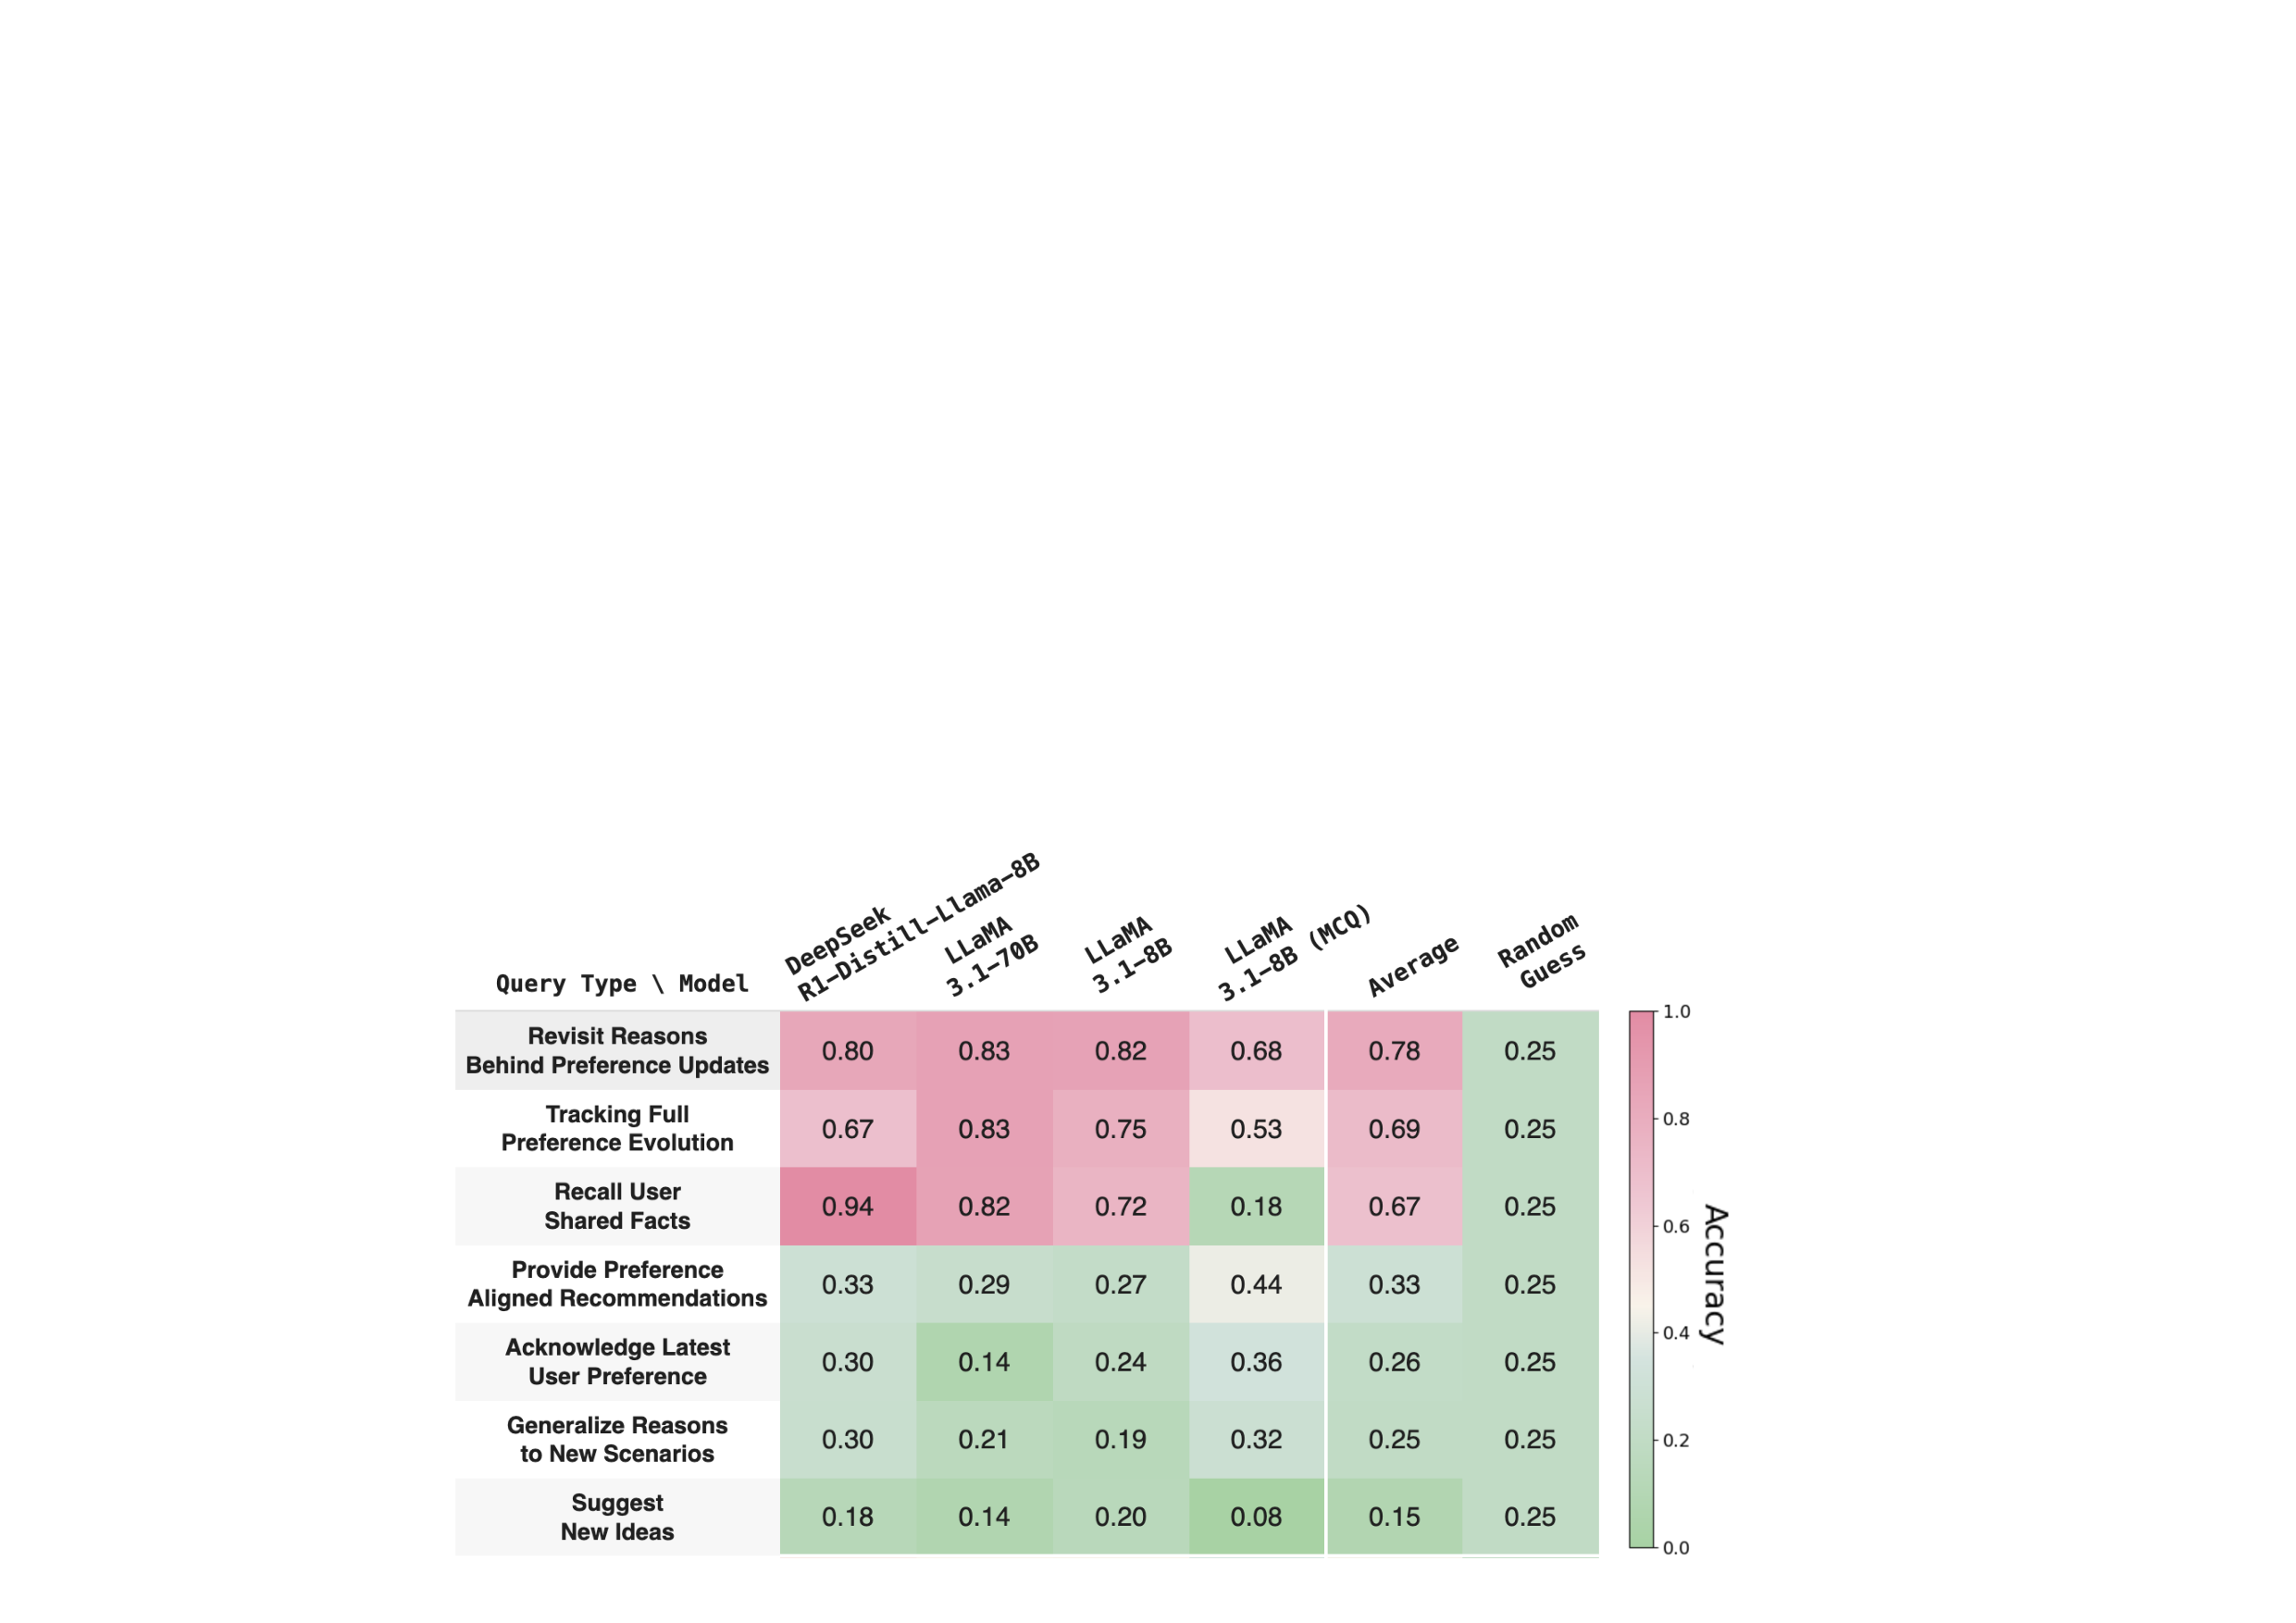
\includegraphics[width=0.53\linewidth]{figures/results_generative.pdf}
  \caption{Generative evaluation on 10-session (32k token length) version of \datasetname.}
  \vspace{-5mm}
  \label{fig:generative}
\end{figure}

% \begin{figure}[t]
%   \centering
%   \includegraphics[width=0.7\linewidth]{Template-2025/figures/results_gen_session.png}
%   \caption{TODO.}
%   % \vspace{-5mm}
%   \label{fig:generative}
% \end{figure}

%often fail to capture the nuanced understanding and reasoning processes underlying each choice. Therefore, we propose the *generative* setting to assess the model's intrinsic confidence and coherence in generating specific responses. This approach not only complements traditional MCQ assessments but also uncovers subtleties in model behavior that may remain hidden when relying solely on discrete answer selections. 
%We have demonstrated the personalization capabilities of LLMs by evaluating their performance on multiple-choice question answering tasks. However, we 